\documentclass[11pt,fleqn]{article}
%\usepackage{CJK}
\usepackage{latexsym}
\usepackage{color}
\usepackage{graphicx, float}\usepackage{graphicx}
%\usepackage[colorlinks]{hyperref}
\setlength{\oddsidemargin}{-0.0in}
\setlength{\evensidemargin}{-0.0in} \setlength{\textwidth}{6.0in}
\setlength{\textheight}{9.0in} \setlength{\topmargin}{-0.2in}

%\setlength{\leftmargin}{0.7in}
\usepackage{amssymb, graphicx, amsmath}  %  fancyheadings,

\newcommand\qed{\qquad $\square$}
\newcommand{\nn}{\nonumber}

\def \[{\begin{equation}}
\def \]{\end{equation}}
\def\proof{{\bf Proof:\quad}}
\def \endzm {\quad $\Box$}
\def\dist{\hbox{dist}}


\newcommand{\R}{\mathbb{R}}
%\newtheorem{yinli}{����}[section]
\newcommand{\D}{\displaystyle}
\newcommand{\T}{\textstyle}
\newcommand{\SC}{\scriptstyle}
\newcommand{\FT}{\footnotesize}



%\newtheorem{theorem}{Theorem}[section]
%\renewcommand{\thetheorem}{\arabic{section}.\arabic{theorem}}
\newtheorem{definition}{Definition}
\renewcommand{\thedefinition}{\arabic{section}.\arabic{definition}}
\newtheorem{lemma}{Lemma}[section]
\renewcommand{\thelemma}{\arabic{section}.\arabic{lemma}}
\newtheorem{remark}{Remark}
\renewcommand{\theremark}{\arabic{section}.\arabic{remark}}
\newtheorem{proposition}{Proposition}[section]
\renewcommand{\theproposition}{\arabic{section}.\arabic{proposition}}
\newtheorem{corollary}{Corollary }[section]
\renewcommand{\thecorollary}{\arabic{section}.\arabic{corollary}}
\renewcommand{\theequation}{\arabic{section}.\arabic{equation}}
\renewcommand{\baselinestretch}{1.35}
\newtheorem{exam}{Example}[section]
\renewcommand{\theexam}{\arabic{section}.\arabic{exam}}
\newtheorem{theo}{Theorem}[section]
\renewcommand{\thetheo}{\arabic{section}.\arabic{theo}}
\begin{document}
%\begin{CJK*}{GBK}{song}

\begin{center}

{\LARGE \bf  Machine Learning and Computer Vision Assignment 1}\\


\vskip 25pt
 {Huihuang Zheng, huihuang@utexas.edu }\\
\vskip 5pt
{\small hz4674 Fall 2015 }


\end{center}

\section{Part 2.5}
\textbf{For following graph, all pictures are ordered by original input, seams, scale resize and seam reduced.} \\
There are 3 successful examples of seam reducing: im1.jpg, im2.jpg and im3.jpg. But im4.jpg and im5.jpg are 2 failed examples. The reason is:
\begin{enumerate}
    \item If image has complex background and simple foreground, the seams in foreground will be removed because of lower energy. For example, the im4.jpg, the woman in green cloth are simple with low gradient. But the forest background has high gradient. So compared to scale resizing, the seam resizing remove a lot of hands and body of the woman. The shape became worse than scale resizing.
    \item For special polygon shapes, like im5.jpg, the seam reducing makes the polygon lose its original shape. But the scaling resizing keeps it well.
\end{enumerate}
\subsection{im1.jpg} Original 600 * 450 image. Reduce height of 50 pixels.
    \begin{center}
        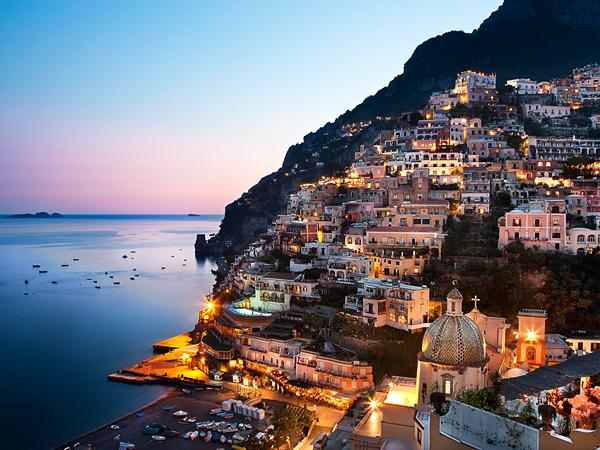
\includegraphics[scale=0.4]{../../output_images/2.5/im1_rh_50_original.jpg}
    \end{center}
    \begin{center}
        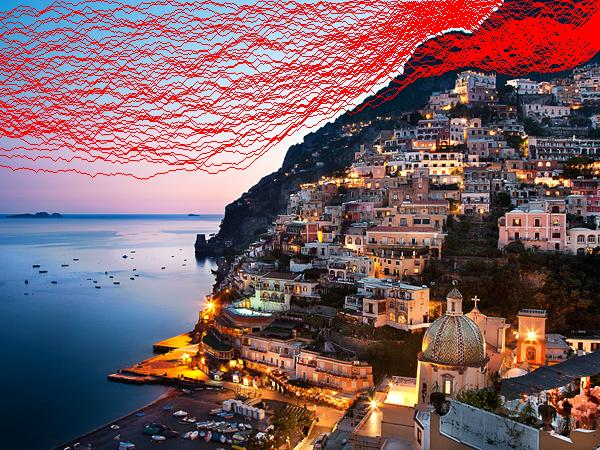
\includegraphics[scale=0.4]{../../output_images/2.5/im1_rh_50_seams.jpg}
    \end{center}
    \begin{center}
        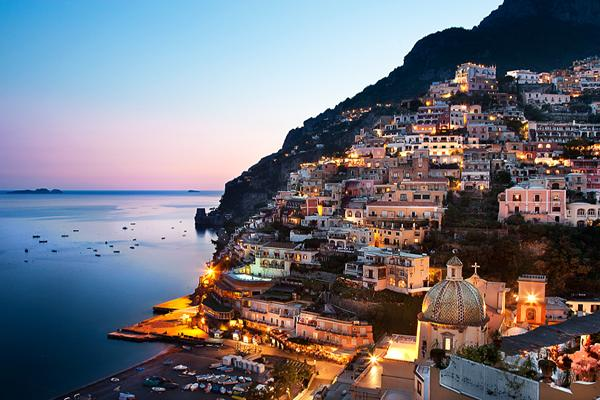
\includegraphics[scale=0.4]{../../output_images/2.5/im1_rh_50_resize.jpg}
    \end{center}
    \begin{center}
        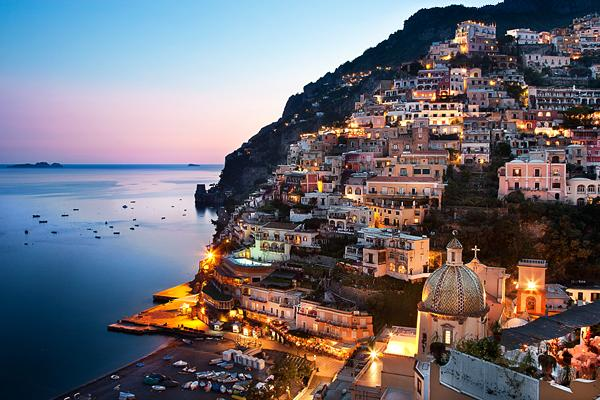
\includegraphics[scale=0.4]{../../output_images/2.5/im1_rh_50_seam_reduce.jpg}
    \end{center}

\subsection{im2.jpg} Original 553 * 369 image. Reduce height of 50 pixels.
    \begin{center}
        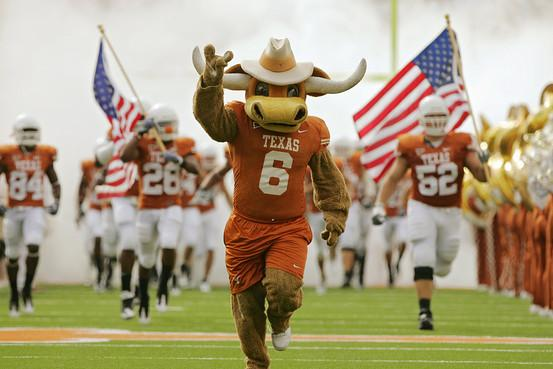
\includegraphics[scale=0.6]{../../output_images/2.5/im2_rh_50_original.jpg}
        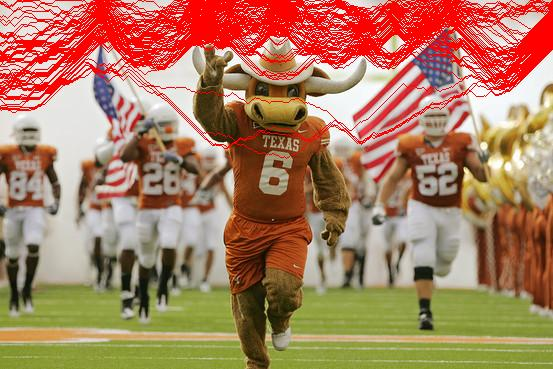
\includegraphics[scale=0.6]{../../output_images/2.5/im2_rh_50_seams.jpg}  
        
\includegraphics[scale=0.6]{../../output_images/2.5/im2_rh_50_resize.jpg}
        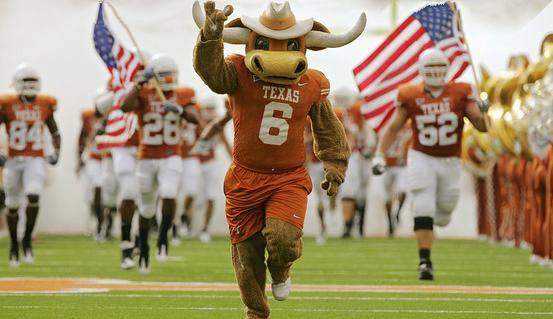
\includegraphics[scale=0.6]{../../output_images/2.5/im2_rh_50_seam_reduce.jpg}
    \end{center}

\subsection{im3.jpg -- a typical successful example} Original 940 * 350 image. Reduce width of 200 pixels.
    \begin{center}
        
\includegraphics[scale=0.4]{../../output_images/2.5/im3_rw_200_original.jpg}
        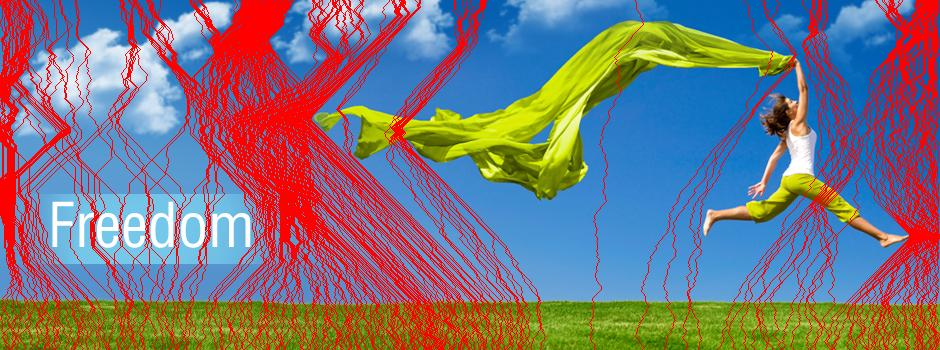
\includegraphics[scale=0.4]{../../output_images/2.5/im3_rw_200_seams.jpg}
        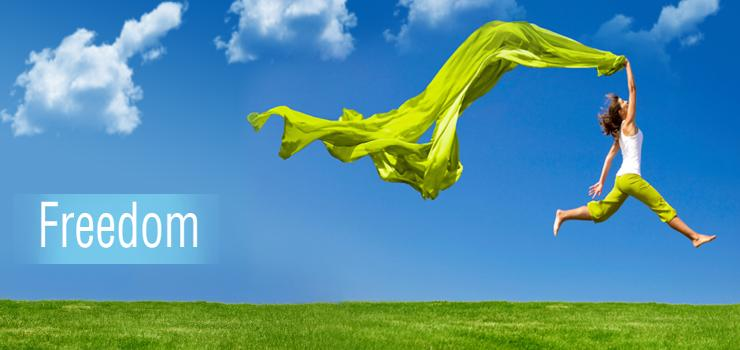
\includegraphics[scale=0.4]{../../output_images/2.5/im3_rw_200_resize.jpg}
        
\includegraphics[scale=0.4]{../../output_images/2.5/im3_rw_200_seam_reduce.jpg}
    \end{center}

\subsection{im4.jpg -- a typical failure} Original 1024 * 680 image. Reduce width of 300 pixels
    \begin{center}
        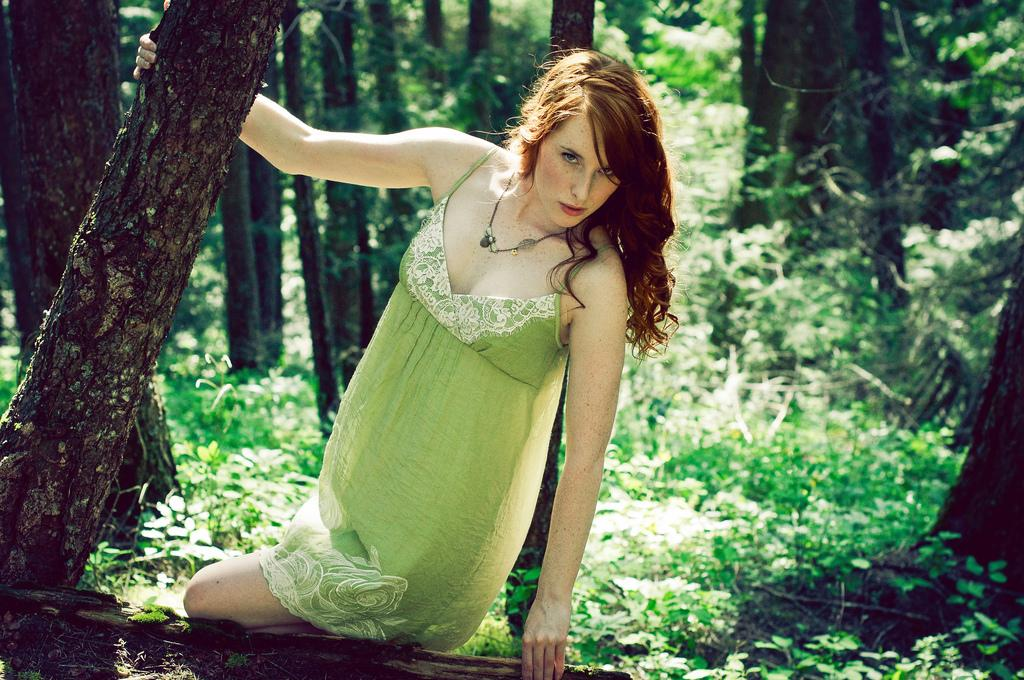
\includegraphics[scale=0.4]{../../output_images/2.5/im4_rw_300_original.jpg}
    \end{center}
    \begin{center}
        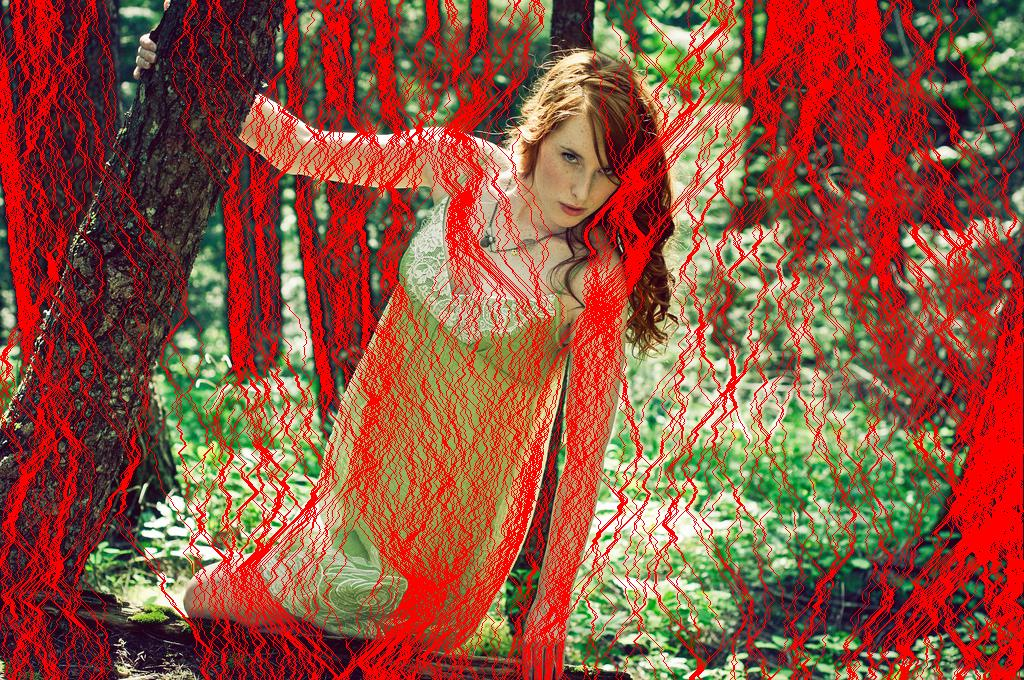
\includegraphics[scale=0.4]{../../output_images/2.5/im4_rw_300_seams.jpg}
    \end{center}
    \begin{center}
        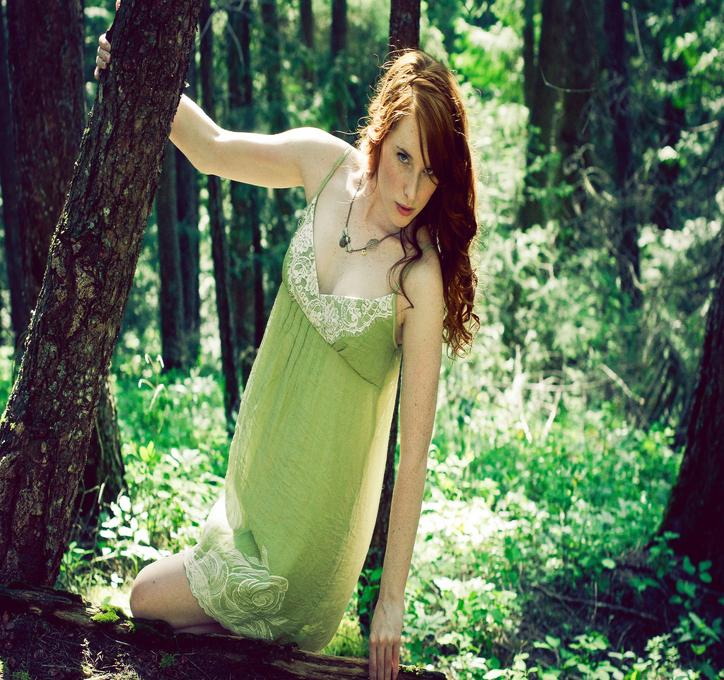
\includegraphics[scale=0.4]{../../output_images/2.5/im4_rw_300_resize.jpg}
    \end{center}
    \begin{center}
        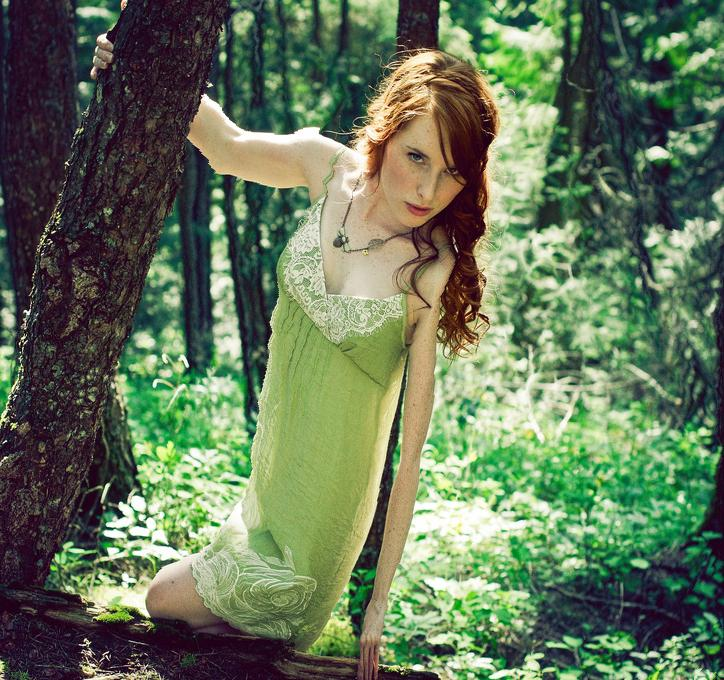
\includegraphics[scale=0.4]{../../output_images/2.5/im4_rw_300_seam_reduce.jpg}
    \end{center}
\subsection{im5.jpg -- second failure example} Original 216 * 233 image. Reduce width of 75 pixels
    \begin{center}
        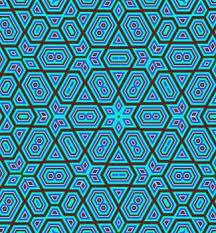
\includegraphics[scale=0.4]{../../output_images/2.5/im5_rw_75_original.jpg}
        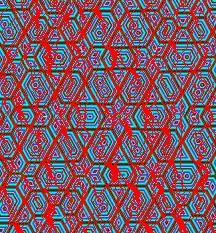
\includegraphics[scale=0.4]{../../output_images/2.5/im5_rw_75_seams.jpg}
        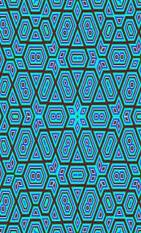
\includegraphics[scale=0.4]{../../output_images/2.5/im5_rw_75_resize.jpg}
        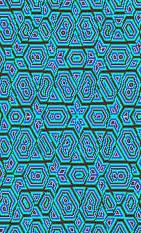
\includegraphics[scale=0.4]{../../output_images/2.5/im5_rw_75_seam_reduce.jpg}
    \end{center}

\section{Extra}
\subsection{Increase Pixels}
To increase pixels, we find the first k seams for removal, and duplicate them by averaging them with their left
and right neighbors (or top and bottom in the horizontal case). 

A example of result: \\
im2.jpg. Original 553 * 369 image. Increase width of 100 pixels.
    \begin{center}
        
\includegraphics[scale=0.6]{../../input_images/im2.jpg}
        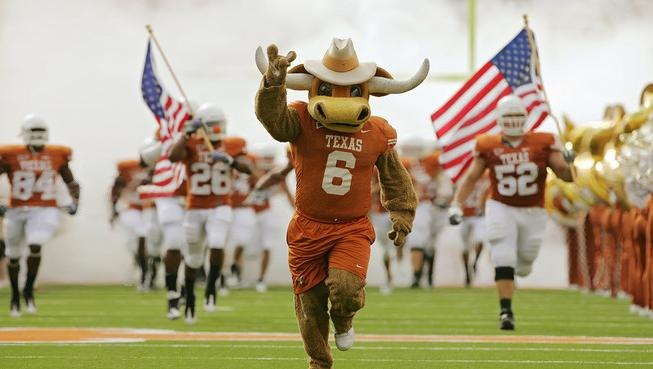
\includegraphics[scale=0.6]{../../output_images/increasePixels/im2_iw_100_seam.jpg}
        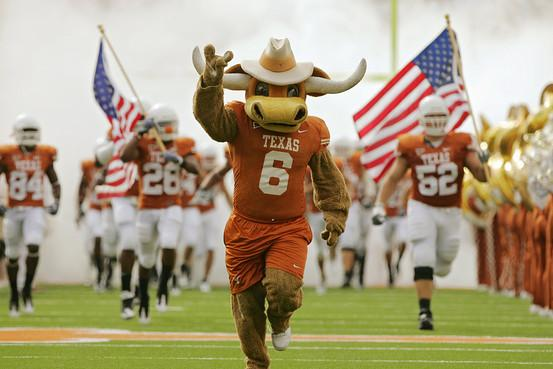
\includegraphics[scale=0.6]{../../output_images/increasePixels/im2_iw_100_resize.jpg}
    \end{center}
\subsection{Remove Object}
Run \emph{removeObject(input\_image)} or \emph{extra()} to see the GUI. Then you can use your mouse to select a polygon region on the image, then my program will remove the object by seaming removing. To remove object, we first computer smaller number of the vertical or horizontal pixels of the target removal region. Then we perform vertical or horizontal removals accordingly. We set the energy in removal region as negative infinite so that the target region will be removed during seam reducing. Since until now, our method doesn't perform Gaussian Blur or something like that to smooth the edge of removal region edge. If you choose something crossing edges. It will be unnatural after removing.\\

A example of result:\\
im2.jpg. Original 553 * 369 image. 
    \begin{center}
        
\includegraphics[scale=0.6]{../../input_images/im2.jpg}
    \end{center}
    Matlab GUI:
    \begin{center}
        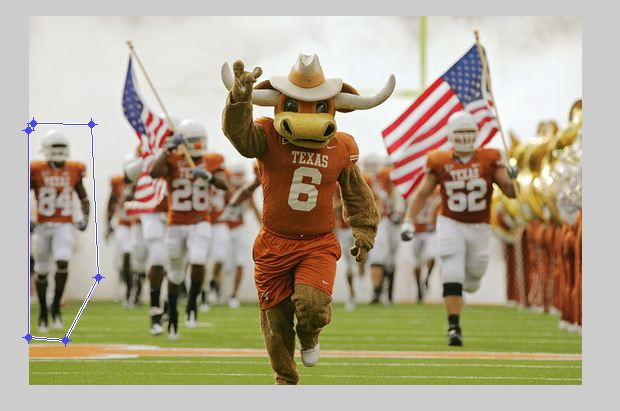
\includegraphics[scale=0.6]{screenShot.jpg}
    \end{center}
    Removed image:
    \begin{center}
        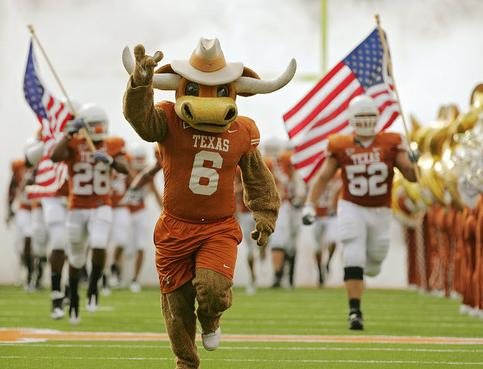
\includegraphics[scale=0.6]{../../output_images/removeObject/im2_ro.jpg}
    \end{center}
    A unnatural example of removing horn:
    \begin{center}
        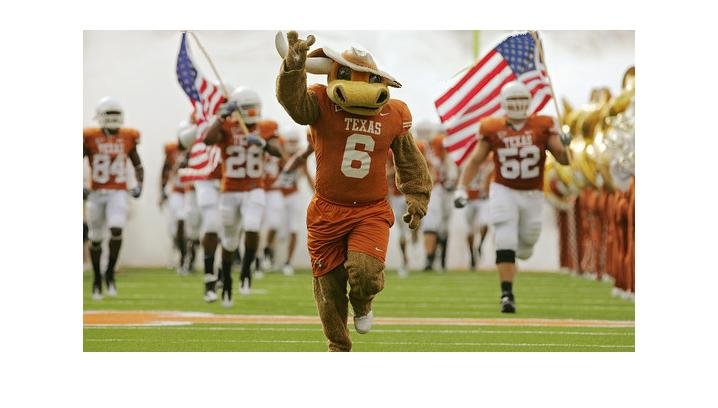
\includegraphics[scale=0.6]{../../output_images/removeObject/unnatural_example.jpg}
    \end{center}
%\end{CJK*}
\end{document}
